% ！注意：编译器需设置为 XeLaTeX
\documentclass[12pt, a4paper, fontset=mac]{ctexart} % 使用ctexart文档类，它天然支持中文并提供了方便的字体命令

% 页面与行距设置
\usepackage{geometry}
\geometry{left=2.8cm, right=2.5cm, top=3.5cm, bottom=2.5cm} % 公文常见页边距，可根据规定调整
\usepackage{setspace}
\onehalfspacing % 设置一倍半行距

% 其他有用的宏包
\usepackage{hyperref}
\usepackage[superscript]{cite}
\usepackage{graphicx}
\usepackage{booktabs}
\usepackage{array}
\usepackage{amsmath,amssymb}
\usepackage{enumitem}

\usepackage{titlesec}
% 恢复到缺省的段落设置
% 标题加粗，与正文在同一行，标题后间距0.5em
\titleformat{\paragraph}[runin]{\normalfont\bfseries}{}{0em}{}
\titlespacing*{\paragraph}{\parindent}{3.25ex plus 1ex minus .2ex}{0.5em}

% 超链接样式
\hypersetup{
    colorlinks=true,
    linkcolor=black, % 公文内部链接常用黑色，更正式
    citecolor=black,
    urlcolor=black
}

\setCJKmainfont{Songti SC}
\setCJKsansfont{Heiti SC}
\setCJKfamilyfont{hei}{Heiti SC}
\setCJKfamilyfont{kai}{Kaiti SC}
\renewcommand{\heiti}{\CJKfamily{hei}}
\renewcommand{\kaishu}{\CJKfamily{kai}}

\usepackage{gbt7714}


% 中文公文样式核心设置：章节标题格式
\ctexset{
    section = {
        format = \zihao{-2} \heiti \centering, % 小二黑体居中 (公文一级标题常用)
        name = {,、}, % 编号格式，如"一、"
        number = \chinese{section}, % 使用中文数字编号
        beforeskip = 24pt, % 段前间距，可根据视觉效果调整
        afterskip = 18pt, % 段后间距
        aftername = \hspace{0.5em} % 编号与标题文字间的距离
    },
    subsection = {
        format = \zihao{-3} \heiti \raggedright, % 三号黑体左对齐 (公文二级标题)
        name = {（,）}, % 编号格式，如"（一）"
        number = \chinese{subsection},
        beforeskip = 18pt,
        afterskip = 12pt,
        aftername = \hspace{0pt}
    },
    subsubsection = {
        format = \zihao{4} \heiti \raggedright, % 四号黑体左对齐 (公文三级标题)
        name = {,．}, % 编号格式，如"1．"
        number = \arabic{subsubsection}, % 三级标题可用阿拉伯数字
        beforeskip = 12pt,
        afterskip = 6pt,
        aftername = \hspace{0pt}
    }
}

% 设置正文默认字号为四号或小三，公文正文常用
\zihao{4} % 或 \zihao{-3}

\title{%
  创新药物研发国家科技重大专项\\[4pt]
  \large 基于真实世界数据构建抗肿瘤药物新药研发与临床试验关键支撑平台\\[8pt]
  \large 项目建议书
}
\author{国家癌症中心}
\date{\today}

\begin{document}
\maketitle

\tableofcontents
\newpage

\section{建议事项概述}

为落实《“健康中国2030”规划纲要》《国家药品安全与高质量发展规划》等重大决策部署，服务国家在抗肿瘤创新药物领域的战略布局，国家癌症中心建议在下一轮“创新药物研发国家科技重大专项”中，\textbf{单列设立}“基于真实世界数据构建抗肿瘤药物新药研发与临床试验关键支撑平台”方向，由国家癌症中心牵头，采用\textbf{国家定向委托方式}组织实施。

\subsection{建议设立的课题方向与组织方式}

\begin{itemize}
  \item 在“创新药物研发国家科技重大专项”总体布局中，建议在“真实世界证据与监管科学”“临床试验效率提升与新范式”“药物全生命周期监管支撑技术”等方向下，\textbf{设立专门任务/定向课题}：
  \begin{quote}
    “基于真实世界数据构建抗肿瘤药物新药研发与临床试验关键支撑平台”。
  \end{quote}
  \item 建议课题采取\textbf{国家定向委托}组织方式，由国家癌症中心牵头，联合相关高校、科研机构、技术企业和创新药企业共同实施。
  \item 建议项目实施周期为\textbf{4年}，总经费建议规模约\textbf{3\,000 万元}人民币，作为创新药物重大专项中肿瘤领域“真实世界证据与监管科学”方向的标志性任务和基础支撑平台。
\end{itemize}

\subsection{项目总体定位与建设内涵}

本项目立足国家癌症中心牵头建设的“国家抗肿瘤药物临床应用监测网”等重大工作基础，覆盖范围包括全国全部肿瘤专科医院以及开展肿瘤诊疗项目的三级综合医院。依托这一平台所整合的全国2\,000余家医院、累计超3\,000 万例肿瘤患者的真实世界诊疗数据，项目将建设一个国家级抗肿瘤药物真实世界数据与真实世界证据（RWD/RWE）基础设施，面向抗肿瘤新药研发与临床试验的全链条需求，提供涵盖数据、方法、工具与标准的一体化支撑。

\vspace{0.5em}
平台拟重点建设：

\begin{enumerate}[label=(\arabic*)]
  \item \textbf{数据标准化治理与专病队列体系}：基于监测网数据，构建覆盖高发及罕见肿瘤、不少于10个细分癌种的标准化专病队列，形成高质量、可溯源的分析级数据资源。
\item \textbf{本土化真实世界评价指标与方法学体系}：结合国际指南与我国临床实践，构建适配本土医疗环境的真实世界总生存期（rwOS）、真实世界无进展生存期（rwPFS）、真实世界客观缓解率（rwORR）等核心终点体系及配套因果推断方法。
  \item \textbf{AI 驱动的数据抽取、质控与队列匹配技术}：研发面向肿瘤领域的医学语言模型、数据质控评分与试验入组/对照匹配算法，实现 RWD 向可审查 RWE 的转化。
  \item \textbf{面向新药全链条的临床试验支撑工具平台}：围绕靶点发现、I--III 期临床试验设计与执行、上市后评价与适应症扩展，构建一系列可配置的支撑工具和服务模块。
  \item \textbf{监管协同与试点应用示范体系}：与药品监管、医保、卫生健康等部门协同，开展若干新药上市/适应症扩展/上市后再评价的试点示范，形成可被监管采信的证据生成路径。
  \item \textbf{产学研用生态与人才培养体系}：建设跨学科复合人才培养机制和“新药研发数据共享协作网络”，推动平台长期可持续运行和行业生态形成。
\end{enumerate}

\subsection{预期贡献及对国家重大需求的支撑作用}

从国家层面看，本项目将：

\begin{itemize}
  \item 为\textbf{创新药物重大专项}提供肿瘤领域“真实世界证据与监管科学”的关键支撑平台，与“基础研究—关键技术—示范应用”总体布局形成良性呼应；
  \item 为国家药监局开展\textbf{真实世界证据审评试点}、制定相关技术指导原则提供实践基础和数据支撑；
  \item 为国家医保局开展\textbf{医保准入评估、支付方式改革和临床价值评估}提供高质量真实世界数据与方法工具；
  \item 为国家卫生健康委推进\textbf{肿瘤规范化诊疗、临床路径优化和癌症防治规划考核}提供连续监测和评估手段；
  \item 通过缩短抗肿瘤新药研发周期、降低单药研发成本、降低临床试验入组难度和罕见癌种试验门槛，\textbf{加快患者获益}，服务“提高五年生存率”等重大健康目标。
\end{itemize}

从实施基础看，国家癌症中心已形成覆盖全国的肿瘤监测网和数据治理体系，具备牵头建设国家级抗肿瘤药物 RWD/RWE 基础设施的\textbf{唯一性和不可替代性}，适宜采用国家定向委托方式组织实施。

\vspace{1em}
\noindent\textbf{说明：}  
以上内容为本项目在创新药物重大专项中拟设立方向及组织方式的\textbf{核心建议}。以下章节为项目建议对应的\textbf{详细设计方案}，供部委相关司局和专家论证参考。

\section{项目背景与战略意义}

\subsection{恶性肿瘤形势与新药研发瓶颈}

当前，恶性肿瘤已成为威胁我国公众健康的重大公共卫生问题，每年新发肿瘤病例超过450万例，死亡病例超过 300 万例，疾病负担持续攀升，严重影响居民健康和社会经济发展\cite{nhc_innovative_drug_guide_2025}。抗肿瘤新药研发需求极为迫切。

近年来，我国创新药研发总体呈现快速发展态势，创新药获批数量稳步提升，部分品种实现与国际同步上市。然而，与欧美发达国家相比，我国仍然面临原始创新能力不足、研发周期长、研发成本高、临床试验效率偏低等突出瓶颈问题\cite{most_guide_2026}。
一方面，高发癌种抗肿瘤药物研发竞争激烈、同质化严重；另一方面，罕见肿瘤和特殊人群药物研发明显不足，临床需求尚未得到有效满足。

临床试验是新药上市的核心环节，也是当前制约我国抗肿瘤新药研发效率和成功率的关键短板之一。传统临床试验模式在实际执行中面临多重困难：晚期肿瘤患者入组难、罕见癌种病例稀缺导致对照设置困难、常见高发癌种对照试验样本量大、成本高、周期长，严重制约新药研发进程\cite{arondekar_oncology_rwe}。

\subsection{真实世界数据与国际发展趋势}

真实世界数据（Real-World Data, RWD）及真实世界证据（Real-World Evidence, RWE）在肿瘤药物研发和监管中的应用，是近年来国际药物研发和监管科学的重要发展方向\cite{sherman_nejm_rwe_2016,concato_nejm_rwe_2022,dang_rwe_primer_2023,costa_frontiers_rwe_2025}。美国 FDA、欧洲 EMA 等监管机构陆续发布系列指导原则，将 RWD/RWE 作为支持新药上市、适应症扩展、上市后再评价的重要证据来源\cite{FDA-RWE-Framework,EMA-External-Control,corrigan_curay_jama_2018,corrigan_curay2018_rwe}。

在抗肿瘤药物领域，国际上已形成较为成熟的 RWD 应用体系：美国已有多个抗肿瘤药物基于 RWD 获批上市或扩展适应症，欧洲约有一定比例的肿瘤药采用基于 RWD 的外部对照用于上市后再评价或适应症扩展\cite{arondekar_oncology_rwe,ECA-Oncology-Review,khozin2017_rwd_oncology,khozin_cancerj_2017,nice_rwd_2025}。Flatiron Health、CancerLinQ 等真实世界肿瘤数据平台，在支持新药研发决策、完善上市后安全性和疗效评价方面发挥了重要作用\cite{flatiron_overview,cancerlinq_overview,ma2020_flatiron_comparison,birnbaum2020_flatiron_cohort}。

我国国家药品监督管理局已发布《真实世界证据支持药物研发与审评的指导原则（试行）》等系列文件，鼓励在药品全生命周期管理中科学合理使用真实世界证据\cite{NMPA-RWE-Guideline,nmpa_rwd_device_2020}，在海南博鳌乐城国际医疗旅游先行区等区域开展了基于 RWD 的真实世界研究试点，为创新医疗器械和部分药品的临床应用与注册提供了有益探索\cite{boao_pilot_rwd,boao_rwd_commentary}。但总体来看，RWD 在抗肿瘤新药研发和临床试验中的系统性应用仍处于起步阶段。

\subsection{我国 RWD 在新药研发中的短板与机遇}

当前我国真实世界数据在抗肿瘤新药研发中的应用仍存在以下突出问题：

\begin{itemize}
  \item \textbf{数据治理不足。} 各级医疗机构 EMR 系统建设不均衡、信息系统异构严重、编码体系不统一，导致数据缺失、噪声较多、可溯源性和可验证性不足。现有数据难以直接支撑跨区域、跨机构的大规模定量分析和严格的因果推断与证据生成。
  \item \textbf{指标体系与方法学尚不完善。} 国际上通行的真实世界总生存期（rwOS）、真实世界无进展生存期（rwPFS）、真实世界客观缓解率（rwORR）等基于真实世界数据判断研究结局终点的方法学指标，是基于欧美人群和医疗体系构建的，需要结合我国诊疗模式与数据特征，构建符合我国国情的真实世界证据评价指标体系和配套方法学框架\cite{hernan_target_trial,makady2017_rwe_def,blonde2018_rwd_rwe,makady_htarwe_2017}。
  \item \textbf{临床、技术与监管协同不足。} 当前真实世界研究大多停留在单点、分散的学术研究和探索性应用层面，尚未形成覆盖药物全生命周期、可持续运行的国家级基础设施。临床一线需求、技术实现路径与监管审评标准之间缺乏系统对接，难以建立可常态化支撑创新药注册与适应症扩展的工作机制\cite{garrison_ispor_2007,berger_ispor_rwd_2017,costa_frontiers_rwe_2025}。
\end{itemize}

与此同时，我国在肿瘤领域真实世界数据资源方面具有独特优势。国家癌症中心近年来牵头建设的肿瘤信息数据库（国家抗肿瘤药物临床应用监测网），基于统一的数据标准和质量控制流程，已累计收录全国 2000 余家医院的肿瘤患者电子病历数据，包括全部肿瘤专科医院和开展肿瘤诊疗的三级综合医院，覆盖超过 3\,000 万例患者，形成了规模全球领先、连续更新的高质量肿瘤真实世界诊疗数据资源\cite{ncc_internal_db,ma_tumor_bigdata_2022}，为构建国家级 RWD 基础设施提供了坚实的数据底座。

本项目拟作为“创新药物研发国家科技重大专项”中\textbf{“真实世界证据与监管科学/临床试验效率提升”方向的重要支撑任务}，依托上述优势，通过建设国家级抗肿瘤药物 RWD/RWE 平台，打通“数据—方法—应用—标准”全链条，填补我国在该领域的关键短板。

\subsection{国家癌症中心的职责使命与现实基础}

国家癌症中心是国家层面肿瘤防治和癌症控制工作的牵头单位，在国家肿瘤监测、临床规范化诊疗、肿瘤防治策略制定和重大专项组织实施等方面承担重要职责\cite{ncc_internal_db,monitoring_network_whitepaper}。近年来，国家癌症中心持续推进“国家抗肿瘤药物临床应用监测网”等重点项目，形成了以下现实基础：

\begin{itemize}
\item \textbf{权威数据源与监测网络。} 监测网自 2018 年启动建设，通过标准化数据模型面向全国 2,000 余家医院持续收集肿瘤患者 EMR 数据，覆盖全国全部肿瘤专科医院及开展肿瘤诊疗项目的三级综合医院。累计收录超过 3,000 万例，涵盖门诊和住院完整诊疗信息，数据连续性、覆盖面和代表性处于国内领先。
  \item \textbf{成熟的数据治理与质控体系。} 在国家科技重大专项等项目支持下，已形成面向肿瘤领域的统一数据标准、清洗流程、质控规范与安全管理制度，为在此基础上进行 RWD/RWE 系统化建设提供了成熟经验。
  \item \textbf{广泛的临床协作网络和多学科专家队伍。} 国家癌症中心联合全国多家三甲医院及专科肿瘤医院，构建了覆盖主要癌种的临床研究协作网络，为 RWD 支撑的新药临床试验设计、执行和验证提供坚实临床基础。
  \item \textbf{与监管和医保部门的协同基础。} 国家癌症中心长期参与国家层面肿瘤防治政策、用药指南及相关技术文件制定，为本项目后续成果转化和纳入监管标准体系提供有利条件。
\end{itemize}

依托上述现实基础，国家癌症中心具备牵头建设国家级抗肿瘤药物 RWD 支撑平台的独特优势，是最适合作为此类国家定向委托项目牵头单位的机构。

\subsection{国内外平台现状与本项目差异化定位}

国际上 Flatiron Health、CancerLinQ 等平台主要基于发达国家医疗体系和支付环境建立，数据结构、指标口径和患者特征与我国存在显著差异\cite{flatiron_overview,cancerlinq_overview,ma2020_flatiron_comparison,birnbaum2020_flatiron_cohort}。这些平台在数据规模、方法学规范和产业协同方面提供了重要借鉴，但难以直接迁移到我国的临床实践与监管场景。

国内方面，国家药监局在真实世界证据政策和区域试点方面已取得积极进展，以海南博鳌乐城为代表的真实世界研究试点逐步探索了 RWD 在医疗器械和部分药品临床评价中的应用路径\cite{NMPA-RWE-Guideline,boao_pilot_rwd,boao_rwd_commentary,nhei_anticancer_eval_guide_2021}。但目前尚缺乏一个在国家层面统一布局、面向肿瘤新药研发与临床试验的高质量真实世界数据关键支撑平台，存在数据源分散、标准不统一、方法学体系不完备、与国家重大专项任务缺乏深度耦合等问题。

本项目的差异化定位在于：立足我国肿瘤防治体系和国家重大专项需求，依托国家癌症中心的权威数据与临床网络，构建\textbf{具有中国特色和国际影响力的抗肿瘤药物 RWD/RWE 国家级基础设施}，实现“数据—方法—应用—标准—产业”的全链条布局，形成可复制、可推广、可对外输出的“中国方案”。

\section{项目总体目标与建设思路}

\subsection{核心目标}

本项目拟依托国家癌症中心肿瘤信息数据库（国家抗肿瘤药物临床应用监测网）以及全国协作医院网络，构建标准化、智能化的\textbf{国家级抗肿瘤药物新药研发与临床试验真实世界数据关键支撑平台}，推动临床试验向“AI+RWD”范式转型，缩短抗肿瘤新药研发周期，降低单药研发成本，为抗肿瘤新药创制提供全流程数据与技术支撑 %\cite{rudrapatna_butte_2020,topol_high_performance_med_2019,kourou_ml_cancer_2015}
。

平台覆盖新药研发各环节，针对性解决不同阶段痛点，实现从早期靶点与候选药物筛选、临床试验设计与执行优化，到上市后疗效与安全性评价的全流程赋能：

\begin{itemize}
  \item 在\textbf{药物遴选与早期研发阶段}，依托海量肿瘤真实世界数据，挖掘肿瘤发病关键机制与潜在靶点，验证候选药物的临床适配性，提升早期研发命中率；
  \item 在\textbf{临床试验阶段}，通过队列匹配、样本量估算、外部对照构建和入组智能匹配等支撑工具，解决入组难、对照设置难和成本高等瓶颈问题，提升试验效率与质量；
  \item 在\textbf{上市后评价阶段}，通过长期随访和真实世界证据生成，为适应症扩展、说明书修订、医保支付和临床指南更新提供有力支撑。
\end{itemize}

\subsection{建设定位与总体架构}

结合创新药物研发国家科技重大专项“基础平台—关键技术—示范应用”整体布局，本项目定位为“国家级抗肿瘤药物 RWD/RWE 基础设施与关键支撑平台”，总体架构可概括为“一平台、三大体系、四类支撑应用”：

\begin{itemize}
  \item \textbf{一平台：} 国家级抗肿瘤药物新药研发与临床试验真实世界数据关键支撑平台，集成数据治理、智能分析、模型开发、协同应用和安全合规等核心能力。
  \item \textbf{三大体系：}
    \begin{enumerate}[label=(\arabic*)]
      \item \emph{数据标准化与质控体系}：面向高发及罕见癌种构建标准化专病队列和统一的数据质量评估体系；
      \item \emph{本土化真实世界评价指标和方法学体系}：构建适配我国人群和临床实践的 RWE 评价指标及配套方法学框架；
      \item \emph{监管协同与标准输出体系}：形成与药品监管、医保支付、临床指南联动的技术标准、白皮书和行业指南。
    \end{enumerate}
  \item \textbf{四类支撑应用：}
    \begin{enumerate}[label=(\arabic*)]
      \item 支撑靶点发现与候选药物筛选；
      \item 支撑 I--III 期临床试验设计与执行；
      \item 支撑上市后疗效与安全性评价与适应症扩展；
      \item 支撑医保支付决策与临床路径优化。
    \end{enumerate}
\end{itemize}

\subsection{实施周期与阶段安排}

结合重大专项整体安排和本项目建设内容的复杂性，建议项目实施周期为\textbf{4 年（3+1 年滚动设计）}，总经费建议规模 3\,000 万元人民币，其中包括数据治理与平台建设、算法研发与算力资源、临床验证与示范应用、标准制定与推广等费用。

\begin{itemize}
  \item \textbf{第一阶段（第 1 年）：} 完成总体方案设计和关键技术路线论证，启动数据标准化治理与专病队列构建，搭建平台原型系统并开展小规模试点。
  \item \textbf{第二阶段（第 2--3 年）：} 在全国范围内推进多癌种专病队列和本土化 RWE 指标体系建设，完成核心算法和工具平台研发，开展 I--III 期临床试验和上市后评价的多点示范应用，初步形成与监管协同的证据生成流程。
  \item \textbf{第三阶段（第 4 年）：} 聚焦“标准化输出与生态构建”，完善技术白皮书和行业指南，形成可复制的应用模式，推动建立全国“新药研发数据共享协作网络”，并拓展国际多中心合作，为后续工程奠定基础。
\end{itemize}

\section{主要建设内容与关键任务}

本项目围绕“数据标准化与质控、本土化指标与方法学、AI 驱动的证据生成技术、监管协同与示范应用”四条主线，部署六大建设任务。

\subsection*{任务一：数据标准化治理与专病队列构建}

依托国家抗肿瘤药物临床应用监测网覆盖全国且持续更新的数千万例肿瘤患者真实世界诊疗数据，运用 AI 大模型及知识图谱等技术，完成多个癌种（包括高发与罕见癌种）的专病队列构建，实现患者基线、诊疗、随访等全维度信息的精准提取和结构化整合\cite{ncc_internal_db}。

\vspace{0.5em}
主要内容包括：

\begin{itemize}
  \item 构建统一的肿瘤领域数据标准和编码体系，涵盖诊断、病理、基因检测、治疗方案、不良反应、随访结局等关键要素；
  \item 利用 NLP 和表型识别技术，从非结构化病历文本中自动抽取关键临床变量，形成结构化数据；
  \item 针对肺癌、乳腺癌、结直肠癌、胃癌等高发癌种，以及胆管癌、胰腺癌等罕见肿瘤构建不少于 10 个细分癌种的专病队列；
  \item 在保证数据安全与隐私保护的前提下，形成覆盖全国、可持续更新的专病队列数据资源，为后续 RWE 研究和临床试验支撑提供数据基础。
\end{itemize}

项目期内，计划纳入总病例数不少于 100 万例分析级病例，每个高发癌种队列病例数不少于 10 万例，罕见癌种队列不少于 5\,000 例，为试验人群筛选和外部对照构建提供充足样本。

\subsection*{任务二：本土真实世界评价指标体系与方法学研发}

借鉴国际通用标准（如 FDA/EMA 指南、ASCO/NCCN 建议等），结合我国临床实践和真实世界数据特征，制定适配本土的真实世界抗肿瘤药物临床试验核心疗效与安全性评价指标体系，形成配套的定义、判读方法和计算标准\cite{hernan_target_trial,arondekar_oncology_rwe}。

\begin{itemize}
  \item 在 rwOS、rwPFS、rwORR 等基础上，提出适合中国人群和诊疗记录特点的本土化指标定义与分层策略；
  \item 建立基于“目标试验（target trial）”框架的 RWE 研究设计和因果推断方法，规范真实世界队列构建和对照选择流程\cite{hernan_target_trial};
  \item 形成覆盖数据清洗、缺失处理、混杂校正、敏感性分析等关键环节的分析方法学规范；
  \item 联合监管和学术组织，发布真实世界肿瘤临床试验评估指标体系和相关技术白皮书、行业指南。
\end{itemize}

\subsection*{任务三：AI 驱动的数据动态提取、质控溯源与匹配预测技术}

研发 AI 驱动的数据动态提取、质控、溯源、匹配、评估与预测的核心算法和技术，在支持海量数据高速处理的基础上，确保数据的准确性、可溯源性和可验证性，为新药研发与临床试验筑牢数据质量基础。

\vspace{0.5em}
主要方向包括：

\begin{itemize}
  \item 针对 EMR 文本和结构化记录，构建面向肿瘤领域的医学语言模型和实体识别模型，实现关键变量自动抽取与语义标准化；
  \item 构建数据质量评估与异常检测模型，形成多维质控评分体系，包括一致性、完整性、可信度等维度；
  \item 研发用于试验入组匹配、对照队列构建的高维相似度匹配与倾向评分算法，支持 I--III 期临床试验的队列筛选和外部对照生成；
  \item 构建数据谱系（lineage）管理与溯源系统，实现从原始数据、清洗转换到分析结果的全流程追踪。
\end{itemize}

\subsection*{任务四：面向临床试验全流程的支撑工具与平台系统}

围绕新药研发各阶段的核心需求，开发一套可配置的临床试验支撑工具平台，重点包括：

\begin{itemize}
  \item \textbf{药物遴选阶段支撑模块：} 面向靶点发现和候选药物筛选，提供靶点–基因–表型–结局关联分析工具，支持未满足临床需求靶点挖掘和人群适配性评估。
  \item \textbf{I 期试验支撑模块：} 基于目标人群基线特征和同类药物真实世界安全性数据，辅助制定入组标准和剂量递增方案，实时监测不良反应与真实世界安全性数据的一致性，降低安全风险。
  \item \textbf{II 期试验支撑模块：} 基于真实世界疗效分布数据和候选药物预期疗效，精准计算样本量，优化目标人群选择，并提供外部对照队列构建功能。
  \item \textbf{III 期试验支撑模块：} 构建覆盖全国的“试验入组智能匹配库”和动态外部对照队列生成工具，提高入组效率，降低对照设置成本，尤其适用于罕见肿瘤临床试验。
  \item \textbf{上市后评价支撑模块：} 支持长期随访队列构建、罕见不良反应信号识别、特殊人群亚组分析等，为适应症扩展、说明书修订和医保支付决策提供依据。
\end{itemize}

以上功能统一集成到平台系统中，面向国家级规模的数据处理和多方协同应用场景。

\subsection*{任务五：监管协同与试点应用示范}

联合国家药监局等监管部门，共同探索 RWD/RWE 在新药研发和审评审批中的应用场景和技术标准，形成“真实世界证据支持创新药注册”的“中国路径”。

\begin{itemize}
  \item 与监管部门共同设计试点示范项目，覆盖新药上市申请、适应症扩展、上市后再评价等典型场景；
  \item 建立真实世界证据生成的标准化流程和审评参考框架，形成监管协同规则和配套工具；
  \item 支持多家创新药企开展基于平台的数据驱动临床试验试点，验证平台在缩短研发周期、降低成本方面的实际成效。
\end{itemize}

\subsection*{任务六：人才培养与产学研用协同生态构建}

依托国家癌症中心及合作高校、科研机构和企业，共同培养“临床研究 + 数据科学 + AI 技术”复合型人才，建设产学研用协同创新生态。

\begin{itemize}
  \item 与高校合作开设“真实世界数据与新药研发”课程，建设联合研究生培养基地；
  \item 建立“新药研发数据共享协作网络”，联合全国医院、科研院所和药企，探索基于联邦学习的数据协同模式；
  \item 推动平台算法和工具产品化，服务更多中小企业和创新团队，降低创新药研发门槛。
\end{itemize}

\section{平台对新药研发全链条的支撑作用}

平台将贯穿“早期研发—临床试验—上市后评价”全链条，为抗肿瘤新药提供系统性支撑。

\subsection{靶点发现与候选药物筛选阶段}

利用大规模真实世界临床数据和随访信息，分析不同人群、不同亚型肿瘤的自然病程和治疗结局，挖掘高未满足临床需求的亚群，识别潜在治疗靶点和适应人群，为药物靶点发现和候选药物筛选提供临床证据基础。

\subsection{I 期临床试验阶段}

通过平台中既有同类药物和类似人群的真实世界安全性数据，辅助制定 I 期试验的入组标准、剂量递增方案和监测指标，识别高风险亚群，优化安全监测策略，降低严重不良事件风险。

\subsection{II 期临床试验阶段}

基于既有治疗模式和真实世界疗效分布，平台可支持 II 期试验的样本量估算、人群分层和终点选择，提升试验设计的科学性和统计效率。借助外部对照队列构建功能，可在特定情形下降低随机对照需求，提高试验可行性。

\subsection{III 期临床试验阶段}

平台通过全国范围的数据覆盖和患者信息整合，为 III 期试验提供大规模入组候选人群，利用智能匹配算法提高入组效率，缩短试验启动和入组周期。同时，通过动态外部对照队列，帮助优化对照方案，尤其在罕见肿瘤、小人群试验中发挥关键作用。

\subsection{上市后评价与适应症扩展阶段}

新药上市后，平台可持续汇聚用药人群的真实世界疗效与安全性数据，构建长期随访队列，识别真实世界中的罕见不良反应和特殊人群获益情况，为适应症扩展、说明书修订和医保支付决策提供系统证据。

\section{数据来源与数据范围}

\subsection{数据来源}

项目数据来源于国家癌症中心肿瘤信息数据库（国家抗肿瘤药物临床应用监测网）。
该数据库自2018年运行，覆盖全国全部肿瘤专科医院及开展肿瘤诊疗的三级综合医院，迄今已积累2,000余家医院、超3,000万例患者的完整EMR数据，
包含门诊及住院完整诊断与治疗信息，数据权威性与完整性得到充分保障\cite{ncc_internal_db}。


所有用于本项目的数据均为脱敏后的去标识化数据，严格符合《个人信息保护法》等相关法律法规要求。数据所有权归国家癌症中心所有，合作单位在项目研究期间仅可在指定的物理隔离、受控环境内使用，确保数据安全与隐私保护。

\subsection{数据范围与规模}

\paragraph{肿瘤类型覆盖。} 重点纳入临床试验需求迫切的癌种，包括肺癌、乳腺癌、结直肠癌、胃癌等高发癌种，以及胆管癌、胰腺癌等罕见肿瘤，构建不少于 10 个细分癌种专病队列。
\paragraph{时间跨度。} 以 2018 年及以后病例数据为起点，在统一标准下对既往与新增病例进行持续滚动汇聚，不预设数据截取的终止时间点，确保数据库动态更新和时效性，支撑疗效与预后相关分析。
\paragraph{数据类型与内容。} 涵盖患者基线信息（年龄、性别、基础疾病、家族史等）、诊疗信息（影像学报告、病理诊断、基因检测结果等）、治疗方案（手术、化疗、放疗、靶向治疗、免疫治疗等）、疗效评估（客观缓解率、疾病控制率等）、不良反应及随访结局（生存状态、复发转移、生活质量等），覆盖临床试验所需的核心变量。
\paragraph{项目期内分析队列规模。} 计划纳入总病例数不少于 1\,000\,000 例分析级病例，每个高发癌种队列病例数不少于 100\,000 例，罕见癌种队列不少于 5\,000 例，同时充分利用监测网超过 3\,000 万例的底层数据资源，为后续多癌种、多场景扩展预留空间。



\section{技术路线与实施路径}

本项目技术路线遵循“数据—模型—应用—标准”的闭环逻辑，重点体现以下特征：

\begin{enumerate}[label=(\arabic*)]
  \item 以国家癌症中心监测网数据为基础，构建统一标准和高质量专病队列（数据层）；
  \item 以 AI 大模型、多模态融合和因果推断方法为核心，形成 RWD 向 RWE 转化的技术引擎（模型层）；
  \item 以新药研发和临床试验关键节点需求为牵引，打造一系列可落地的支撑工具和平台系统（应用层）；
  \item 以监管和临床指南为抓手，形成标准化的证据生成和应用路径，反哺数据和模型持续迭代（标准层）。
\end{enumerate}

\begin{figure}[htbp]
  \centering % 替换了原来的 center 环境，确保内容居中
  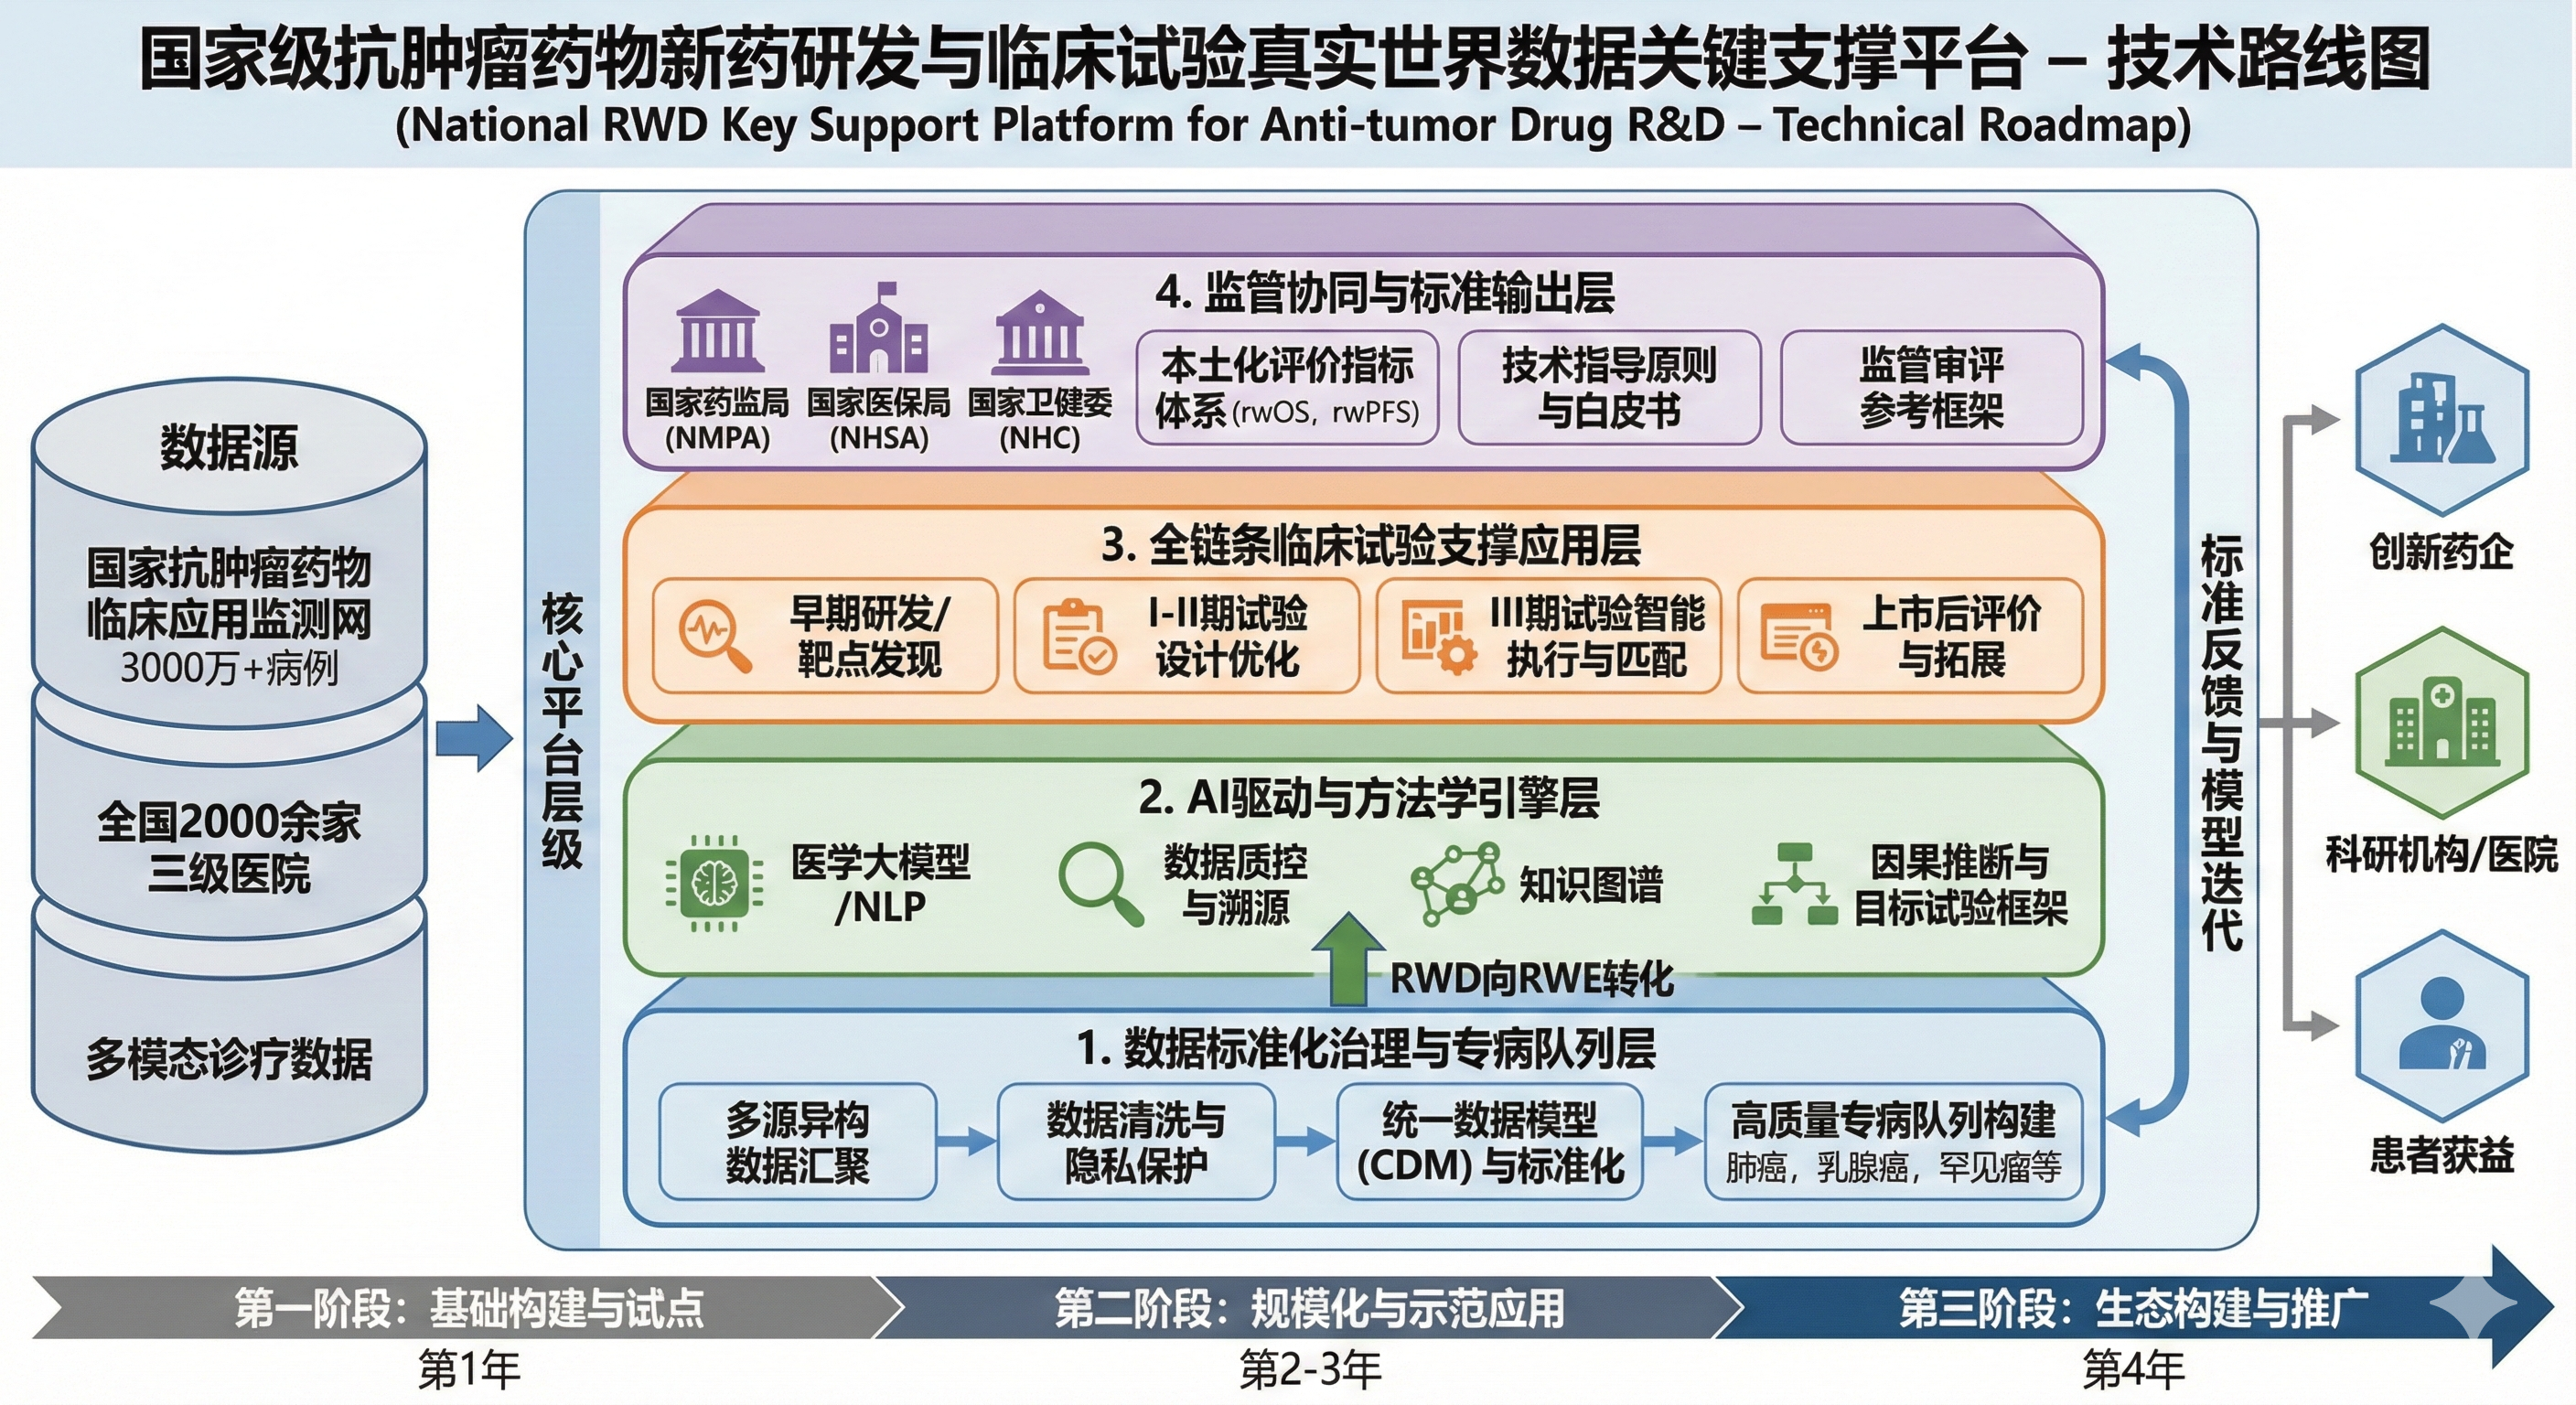
\includegraphics[width=0.9\textwidth, keepaspectratio]{1.png}
  \caption{项目总体技术路线示意图}
  \label{fig:tech_route}
\end{figure}

在实施路径上，将采用“示范先行—标准固化—协作网络推广”的逐步推进策略：优先围绕若干高发癌种完成端到端闭环示范，再逐步扩展到罕见癌种和特殊人群，同时通过协作网络机制和联邦学习技术实现全国范围内的数据协同和标准推广。

\section{组织实施与合作模式}

\subsection{各方角色分工}

\paragraph{国家癌症中心（牵头单位）。} 作为项目牵头单位，承担整体组织协调和质量控制职责，负责临床需求定义、权威数据供给、伦理审查、临床验证与监管协同工作，牵头制定行业指南与技术白皮书，保障项目的临床适用性与权威性。

\paragraph{技术合作企业。} 负责 AI 算法研发、平台搭建、数据标准化处理与本土指标技术实现，提供数据安全防护技术支撑，保障平台技术先进性与安全性。

\paragraph{药企（应用与参与方）。} 利用平台资源优化新药研发策略和临床试验设计、降低研发成本，参与试点验证并反馈应用需求，形成“研发—验证—迭代”的良性循环。

\subsection{合作模式与治理机制}

项目遵循“医研协同、数据驱动、合规可控、共研共享”原则，拟成立由国家癌症中心牵头、监管部门指导、技术企业和药企参与的联合课题组，建立“临床需求牵引、技术支撑保障、监管全程协同”的运作机制，确保项目高效推进与成果落地。

在治理机制上，将设立项目专家委员会和数据与伦理委员会，分别负责重大技术路线、临床试验方案的论证以及数据安全、伦理合规的审查，为项目顺利实施提供制度保障。

\section{关键指标、风险与合规保障}

\subsection{关键建设与应用指标}

结合项目目标，拟设置以下几类关键指标：

\begin{itemize}
  \item \textbf{数据资源与平台建设指标}
    \begin{itemize}
      \item 建成 1 个国家级抗肿瘤药物新药研发与临床试验真实世界数据关键支撑平台；
      \item 构建不少于 10 个细分癌种的标准化专病队列，总病例规模达百万例以上；
      \item 数据覆盖临床试验核心变量数达到规定要求。
    \end{itemize}
  \item \textbf{技术与标准成果指标}
    \begin{itemize}
      \item 形成 AI 驱动的数据治理、动态匹配、质控溯源等核心算法模型若干项；
      \item 获得相关软件著作权或专利若干项；
      \item 制定真实世界肿瘤临床试验评估指标体系，发布若干技术白皮书和行业指南。
    \end{itemize}
  \item \textbf{应用示范与监管协同指标}
    \begin{itemize}
      \item 支持多家创新药企开展基于平台的新药研发与临床试验试点应用；
      \item 每年支撑一定数量的新药相关申报事项通过监管审评；
      \item III 期临床试验入组周期缩短、单药研发成本降低等关键效益指标达到预期。
    \end{itemize}
  \item \textbf{人才与生态指标}
    \begin{itemize}
      \item 联合培养跨领域复合型专业人才若干名；
      \item 建立覆盖全国的新药研发数据共享协作网络，通过联邦学习等技术实现病例总数达千万例以上的数据协同。
    \end{itemize}
\end{itemize}

\subsection{风险分析与应对策略}

\paragraph{数据质量与代表性风险。}  
\emph{风险：} 各医疗机构数据质量存在差异，部分变量缺失和偏倚可能影响研究结论的可靠性。  
\emph{对策：} 通过统一数据标准、严格质控体系和多维度质量评分系统，对数据进行分层使用；对重要分析采用敏感性分析和多种方法学交叉验证，提升结论稳健性。

\paragraph{方法学与监管认可风险。}  
\emph{风险：} 新的 RWE 方法和指标体系能否被监管部门和学术界广泛认可存在不确定性。  
\emph{对策：} 全程加强与监管部门、专业学会和国际同行的互动，在试点项目中积累经验，逐步固化为指南和技术白皮书，形成可被审评接受的标准路径。

\paragraph{数据安全与隐私保护风险。}  
\emph{风险：} 大规模真实世界数据的集中处理和分析存在潜在信息泄露风险。  
\emph{对策：} 严格落实《个人信息保护法》等法律法规要求，采用数据脱敏、访问控制、物理隔离、可信执行环境等多重技术手段，必要时采用联邦学习等新型隐私保护技术，加强安全审计和应急预案。

\paragraph{多方协同与可持续运行风险。}  
\emph{风险：} 项目涉及国家级机构、监管部门、医院、企业等多方，协同复杂，长期运行和维护存在不确定性。  
\emph{对策：} 明确权责分工，建立科学的利益分配机制和持续更新的服务模式（如平台服务、数据服务、技术转化），增强平台可持续运营能力。

\section{建议采取国家定向委托方式实施的理由}

本项目具有以下特点：

\begin{itemize}
  \item \textbf{重大国家战略需求导向。} 针对我国抗肿瘤新药研发周期长、成本高和临床试验效率低等重大瓶颈问题，以国家级 RWD/RWE 基础设施建设为抓手，直接服务创新药物研发国家科技重大专项总体目标。
  \item \textbf{强数据主权与安全合规要求。} 项目涉及覆盖全国的肿瘤患者真实世界诊疗数据，属于重要数据和敏感个人信息范畴，必须在国家主导、权威机构牵头的框架下统一规划和安全管理。
  \item \textbf{需要权威机构统筹临床与监管资源。} 只有以国家癌症中心为牵头单位，才能统筹全国临床协作网络和监管资源，形成“临床需求—技术方案—监管标准”一体化闭环。
  \item \textbf{技术复杂度高、生态协同度要求高。} 平台建设涉及 AI 大模型、因果推断、隐私计算、多机构数据协同等前沿技术，同时需要协调医院、企业和高校等多方参与，适合由国家级机构在国家重大专项框架下定向组织实施。
\end{itemize}

因此，建议将“基于真实世界数据构建抗肿瘤药物新药研发与临床试验关键支撑平台”纳入创新药物研发国家科技重大专项，采用\textbf{国家定向委托方式}，由国家癌症中心牵头组织实施，联合相关部委、科研机构和企业共同完成。

\section{预期经济社会效益与中长期拓展}

项目建成后，将在以下几个方面产生显著的经济社会效益：

\begin{itemize}
  \item \textbf{显著降低抗肿瘤新药研发成本，提升研发效率。} 通过真实世界数据支撑靶点验证、试验设计和外部对照构建，可缩短临床试验周期，降低样本量和对照设置成本，降低单药研发总体投入。
  \item \textbf{降低创新门槛，激发产业创新活力。} 为中小企业和初创企业提供高质量数据和技术支撑，降低其开展创新药研发的门槛，带动国内抗肿瘤创新药研发投入整体增长，促进医药产业高质量发展。
  \item \textbf{加速患者获益，助力“健康中国2030”目标。} 通过缩短创新药上市时间和扩展适应症，使更多肿瘤患者更早用上安全有效的创新药物，为提升我国癌症 5 年生存率目标提供有力支撑。
  \item \textbf{提升我国在全球药物研发领域的话语权。} 作为自主可控的国家级抗肿瘤药物创新体系核心基础设施，平台将填补我国在真实世界数据支撑新药研发领域的空白，有望在国际 RWD/RWE 标准制定中输出中国经验，提升我国在全球药物研发领域的影响力。
\end{itemize}

在中长期，本项目将以数据资源平台为核心基础，围绕肿瘤药物研发全链条需求，逐步构建“数据—技术—应用—产业”的完整生态体系，发展新药研发数字化基础设施与服务体系，形成可持续演进的国家能力，为后续更多重大专项任务和国家战略布局提供可复用、可扩展的技术与数据底座，逐步在全球真实世界证据支持的新药研发领域形成具有国际影响力的“中国方案”。

\section{结语与工作建议}
综上所述，国家癌症中心建议：在下一轮“创新药物研发国家科技重大专项”总体布局中，\textbf{单列设立}“基于真实世界数据构建抗肿瘤药物新药研发与临床试验关键支撑平台”相关任务，采用\textbf{国家定向委托方式}，由国家癌症中心牵头组织实施，联合相关高校、科研机构、技术企业和创新药企业共同推进。

本项目将以国家癌症中心已建成的全国肿瘤监测网络和真实世界数据资源为基础，面向抗肿瘤新药研发和临床试验全链条需求，构建我国抗肿瘤药物 RWD/RWE 的国家级基础设施，为提升我国创新药物研发能力、加快创新药物临床转化和患者可及性、服务“健康中国2030”战略目标提供有力支撑。

国家癌症中心将在相关部委指导下，进一步细化和优化任务方案、技术路线与实施路径，主动对接创新药物研发国家科技重大专项总体部署和相关方向安排，确保项目一经立项即可平稳、有序、高质量推进。

\vspace{1em}
\bibliographystyle{gbt7714-numerical}
\bibliography{refs}
\end{document}
